\chapter{技術記事のまとめ}

\begin{tcolorbox}[title=お品書き]
  \begin{itemize}
    \item p.7 『DiscordBot を作ってみよう』suda
          似たような会話をするのが煩わしいので自分っぽい反応をするDiscordBotを作ってみました!
    \item p.11『DiscordBot を作ってみよう』hihumikan
          Git初心者に向けたGitで使えると嬉しいことをまとめました!
    \item p.16『Gin × Neo4j × Docker で最短経路を返す API サーバを建てる』水谷
          グラフDBであるNeo4jとGo(Gin)を用いた経路探索APIと、そのAPIサーバを構築します!!
    \item p.29『Next.js 13 触ってみた』Beyond Toyama
          最新のNext.js 13になったことで追加された機能や変更された部分を紹介しています!
  \end{itemize} 
\end{tcolorbox}

% \begin{figure}[H]
%   \centering
%   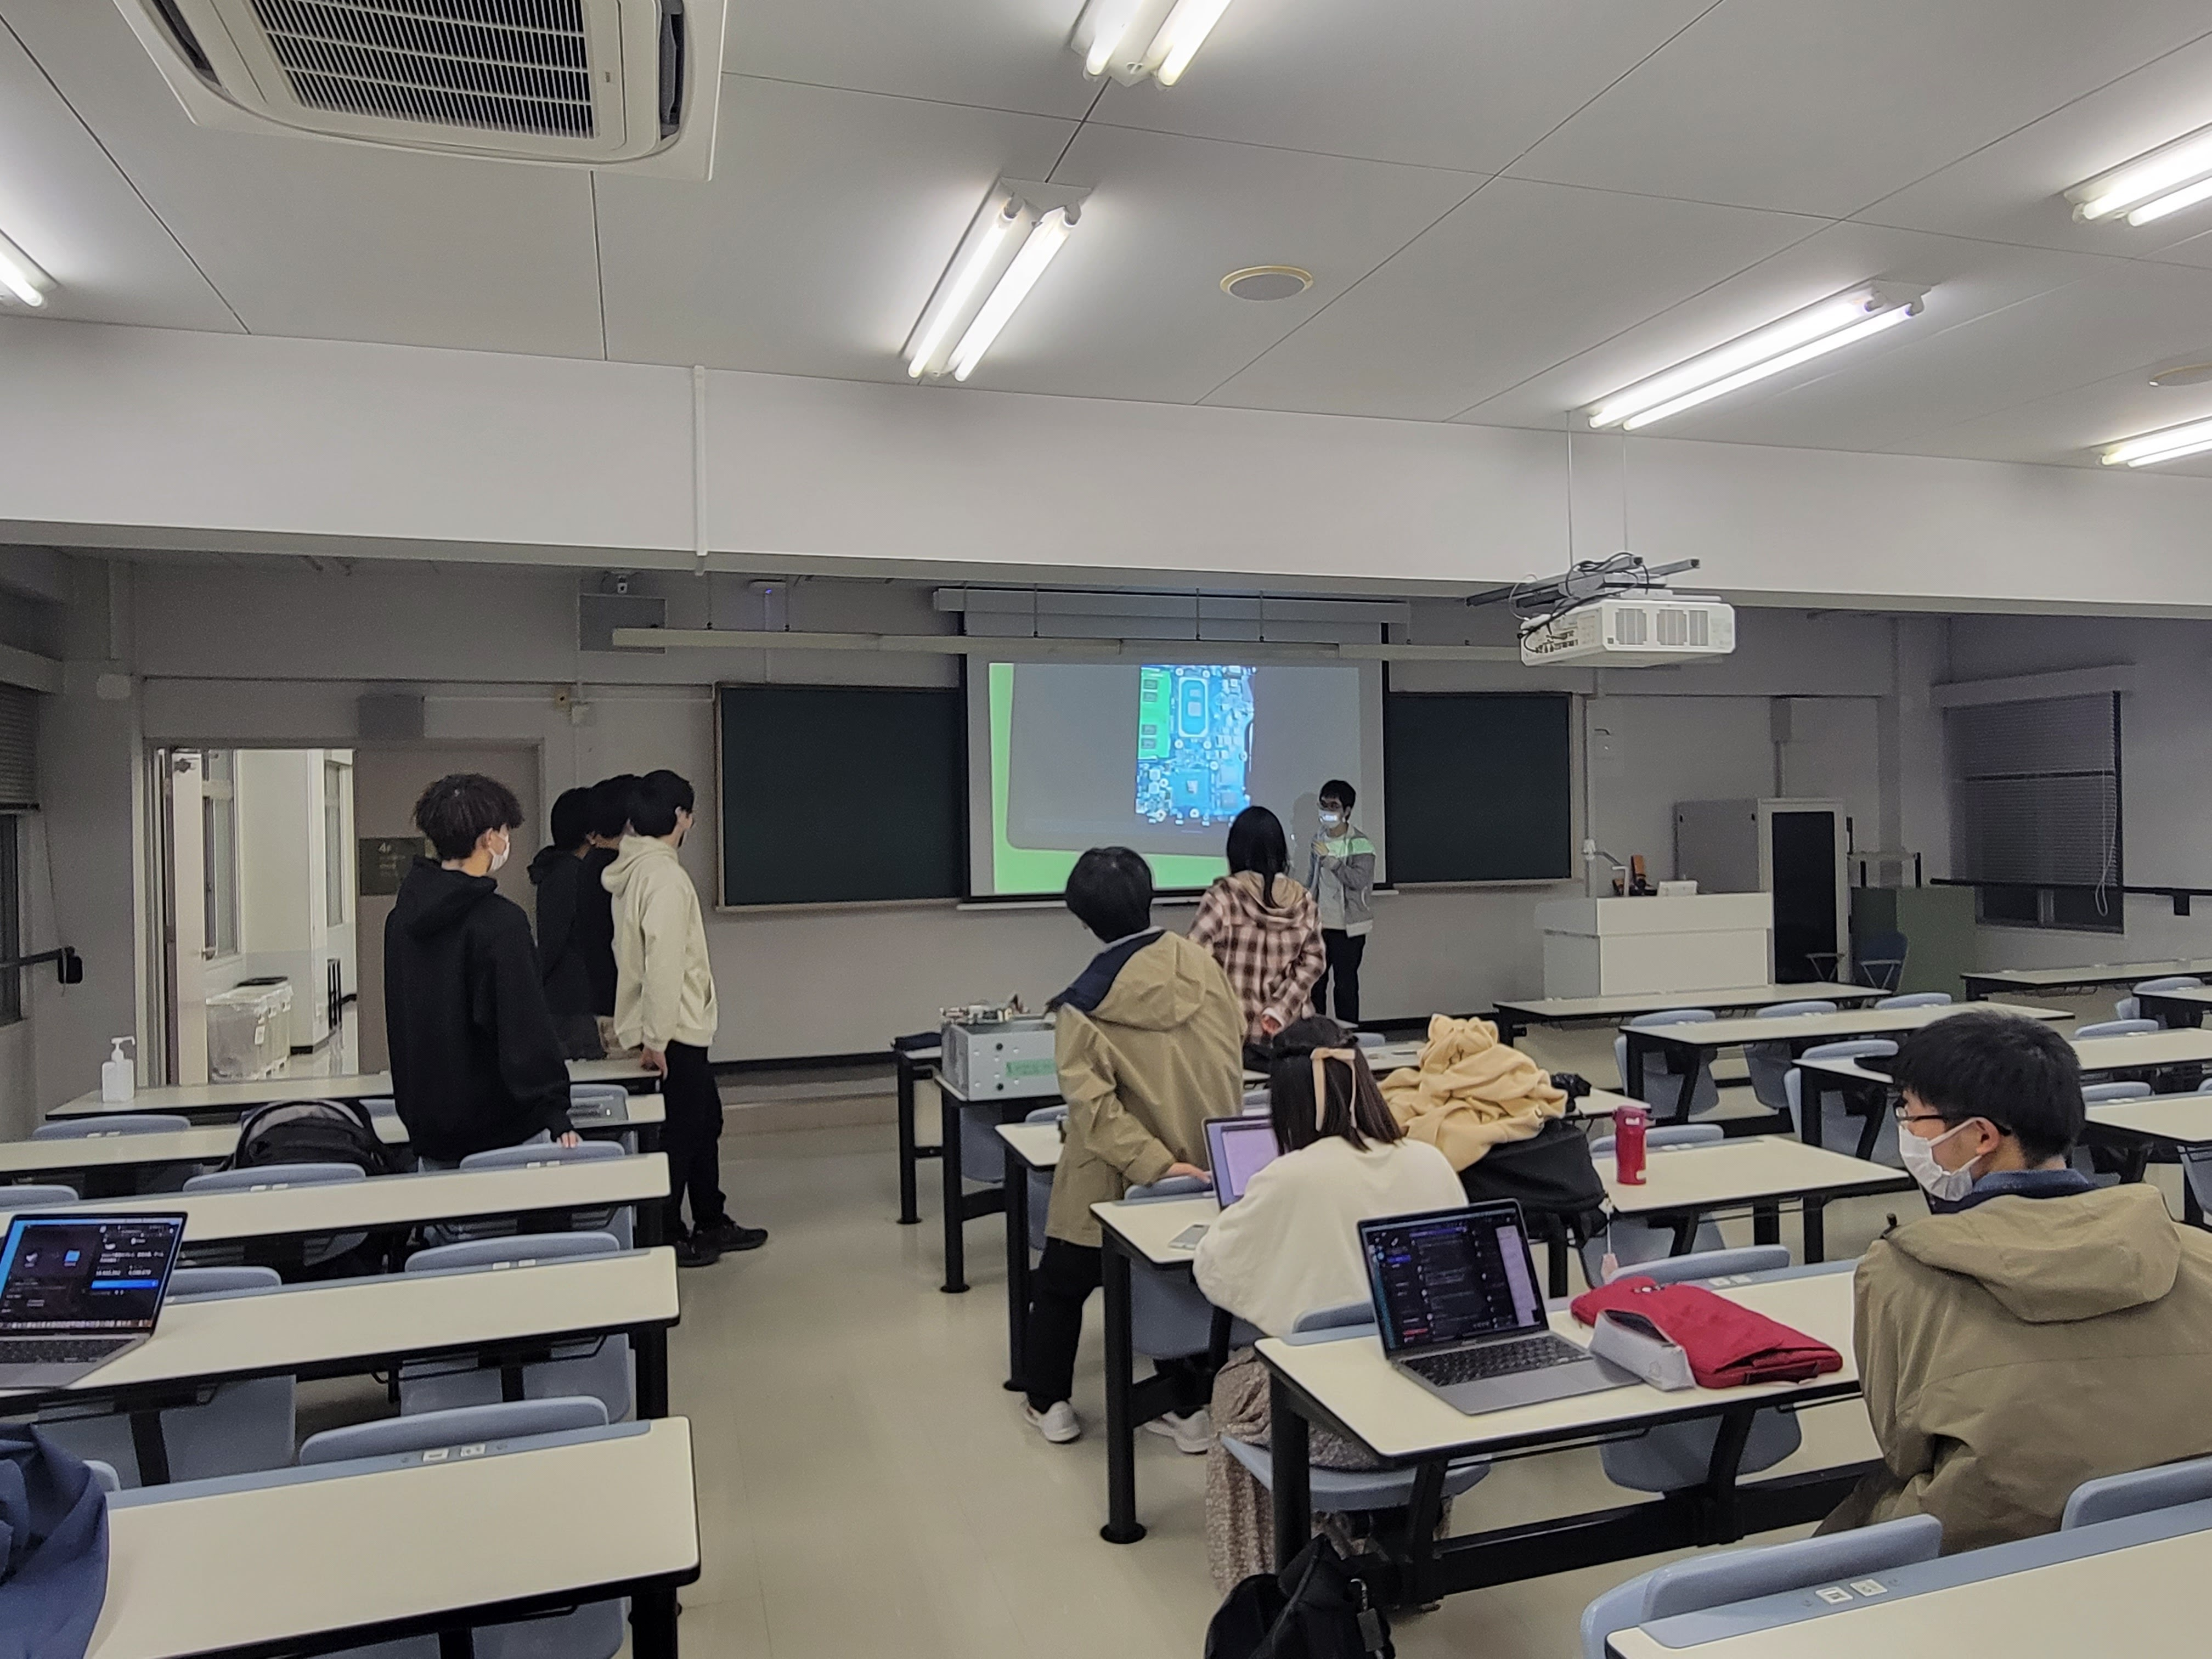
\includegraphics[width=6cm]{./image/03-Tech/benkyoukai.jpg}
%   \caption{シス研で勉強会を行っている様子}
%   \label{benkyoukai}
% \end{figure}